\documentclass[12pt]{article}
\usepackage[latin9]{inputenc}
\usepackage{geometry}
\geometry{verbose}
\usepackage{amsmath}
\usepackage{amssymb}
\usepackage{setspace}
\usepackage{natbib}
\setcitestyle{aysep={}}

\makeatletter

%%%%%%%%%%%%%%%%%%%%%%%%%%%%%% User specified LaTeX commands.

\usepackage{amsthm}\usepackage{epsfig}\usepackage{psfrag}\usepackage{lineno}


%\setlength{\evensidemargin}{0in} \setlength{\oddsidemargin}{0in}
%\setlength{\topmargin}{0.0in} \setlength{\textwidth}{6.5in}
%\setlength{\textheight}{9in} \setlength{\topskip}{0in}
%\setlength{\headheight}{0in} \setlength{\headsep}{0in}
\usepackage[labelfont=bf,labelsep=period]{caption}

\makeatother

\usepackage{Sweave}
\begin{document}
\input{multimark-concordance}
%\SweaveOpts{concordance=TRUE}
%% TITLE %%%%%%%%%%%%%%%%%%%%%%%%%%%%%%%%%%%%%%%%%%%%%%%%%
\global\long\def\baselinestretch{1.8}


\begin{center}
\texttt{\LARGE multimark}{\LARGE : an R package for analysis of capture-recapture data consisting of multiple ``non-invasive'' marks}\vspace{0.5in}

\par\end{center}

\begin{center}
{\large Brett T. McClintock$^{1}$} 
\par\end{center}



\begin{center}
\hrulefill{} 
\par\end{center}

\begin{center}
\global\long\def\baselinestretch{1.25}
 {\large National Marine Mammal Laboratory}
\par\end{center}{\large \par}

\begin{center}
{\large Alaska Fisheries Science Center}\\
 {\large {} NOAA National Marine Fisheries Service}\\
 {\large {} Seattle, Washington, U.S.A.}\\
 {\large {} $^{1}${\em Email:} brett.mcclintock@noaa.gov} 
\par\end{center}



\begin{center}
{\large \hrulefill{}} 
\par\end{center}

\begin{center}
\textsc{Running Head}: \verb|multimark| mark-recapture package \bigskip{}

\par\end{center}

\begin{center}
May 11, 2015 
\par\end{center}

\clearpage{}

\setlength{\textheight}{575pt} \global\long\def\baselinestretch{2}
 %% ABSTRACT %%%%%%%%%%%%%%%%%%%%%%%%%%%%%%%%%%%%%%%%%%%%%%%%%%%%%


%  make sure that the document has 25 lines per page (it is 12 pt)
\setlength{\textheight}{575pt} \setlength{\baselineskip}{24pt} %think this may do doublespacing (required for submission I think)

\newpage{}

\noindent \textbf{Summary}\\
\textbf{1.} I describe an open source R package, \verb|multimark|, for estimation of survival and abundance from capture-mark-recapture data consisting of multiple ``non-invasive'' marks. Non-invasive marks include natural pelt or skin patterns, scars, and genetic markers that enable individual identification in lieu of physical capture, and thus apply to any species that can be individually identified from visual or genetic sampling surveys. \verb|multimark| provides a means for combining and jointly analyzing encounter histories from multiple non-invasive sources that otherwise cannot be reliably matched (e.g. left- and right-sided photos of bilaterally asymmetrical individuals). \\
\textbf{2.} \verb|multimark| is currently capable of fitting open population Cormack-Jolly-Seber
(CJS) and closed population abundance models with two mark types using Bayesian Markov chain Monte Carlo (MCMC) methods. \\
\textbf{3.} Some package features include: (i) general model specification using formulas already familiar to most R users, (ii) ability to include temporal, behavioural, cohort, and individual heterogeneity effects in detection and survival probabilities, (iii) Bayesian multimodel inference using reversible jump MCMC, and (iv) data simulation capabilities for power analyses and assessing model performance. \\
\textbf{4.} I demonstrate use of \verb|multimark| using left- and right-sided encounter histories for bobcats (\textit{Lynx rufus}) collected from remote single-camera stations in southern California. In this example, there is evidence of a behavioural effect (i.e. trap ``happy'' response) that is otherwise indiscernible using traditional single-sided analyses.\\
\textbf{5.} The package will be most useful to ecologists seeking to combine different sources of mark-recapture data that are difficult (or impossible) to reliably reconcile, particularly with the sparse datasets typical of rare or elusive species for which non-invasive sampling techniques are most commonly employed. \\


\noindent \textbf{Key-words} Bayesian multimodel inference, capture-recapture, Cormack-Jolly-Seber (CJS), latent multinomial, mark-recapture, Markov chain Monte Carlo (MCMC), multiple lists, population size

%\newpage{}

\linenumbers

\global\long\def\baselinestretch{1.0}
 \global\long\def\baselinestretch{1.0}


\section{Introduction}

``Non-invasive'' capture-recapture sampling techniques are becoming commonplace for monitoring animal populations \citep[e.g.][]{Hammond1990,LukacsBurnham2005a,OConnellEtAl2010}. Examples of non-invasive marks include natural pelt or skin patterns, scars, and genetic markers that enable individual identification in the absence of physical capture. Capture-recapture methods based on non-invasive marks have been applied to diverse taxa, including sharks \citep[e.g.][]{HolmbergEtAl2008}, reptiles \citep[e.g.][]{NairEtAl2012}, ursids \citep[e.g.][]{DreherEtAl2007}, felids \citep[e.g.][]{KaranthNichols1998,RuellEtAl2009}, and marine mammals \citep[e.g.][]{Hammond1990,WilsonEtAl1999,MadonEtAl2011}. While non-invasive capture-recapture methods have many advantages related to financial cost and animal welfare, they also pose new difficulties such as animal misidentification \citep{WrightEtAl2009,YoshizakiEtAl2009,LinkEtAl2010,MorrisonEtAl2011} and the complexity of multiple types of marks \citep{CorkreyEtAl2008,MadonEtAl2011,BonnerHolmberg2013,McClintockEtAl2013a}. 

Multiple marks can arise from sighting or camera surveys of species with natural mark patterns that are bilaterally asymmetrical (e.g. cetaceans, felids) or from multiple sources of non-invasive capture-recapture data being collected concurrently (e.g. faecal DNA sampling and visual surveys). With multiple marks, an encounter history is produced for each individual and mark type, but there is typically no reliable means to match them (unless each mark type is simultaneously observed at least once for every encountered individual). Because the number of unique individuals encountered must be known for standard capture-recapture analyses of population abundance (or related demographic parameters), the typical approach is to conduct separate analyses for each mark type and compare the results \citep[e.g.][]{WilsonEtAl1999,BerrowEtAl2012,NairEtAl2012}. However, given that sample sizes (and precision) may be considerably reduced, this is not as efficient as conducting an integrated analysis utlizing encounter histories arising from all mark types \citep{McClintockEtAl2013a}. Additional costs of conducting separate analyses for each mark type include a limited ability to explore models with behavioural or cohort effects, and, for capture-recapture models that condition on first encounter, a forfeiting of information from histories with the (apparent) first encounter occurring on the last sampling occasion. These limitations can be particularly important for the sparse datasets typical of rare and elusive populations for which non-invasive sampling techniques are most commonly employed. 

\cite{BonnerHolmberg2013} and \cite{McClintockEtAl2013a} recently developed methods for performing integrated analyses of capture-recapture data consisting of multiple non-invasive marks. However, to my knowledge, their approaches have yet to be applied by practitioners. This is certainly not due to a lack of appropriate data \citep[e.g.][]{WilsonEtAl1999,HolmbergEtAl2008,MadonEtAl2011,BerrowEtAl2012,NairEtAl2012}, and is likely attributable to the mathematical and computational complexity of the models, as well as a lack of user-friendly software for implementing them. This is the motivation for \verb|multimark|, an R \citep{RTeam2013} package for the analysis of capture-recapture data consisting of multiple non-invasive marks. 

After providing some additional background on capture-recapture with multiple marks, I briefly describe the models implemented in \verb|multimark|. These currently include open population Cormack-Jolly-Seber (CJS) and closed population abundance models \citep[e.g.][]{WilliamsEtAl2002} with two mark types. Using real and simulated data for illustration, I provide an overview of the workflow for the package and a new analysis of left- and right-sided encounter histories for bobcats ({\it Lynx rufus}) collected from remote single-camera stations in southern California. Additional information, including help files, data, examples, and package usage is available by downloading the \verb|multimark| package from CRAN (http://cran.r-project.org) or github (https://github.com/bmcclintock/multimark).

\section{Description}
\subsection{Background}

Capture-recapture data are typically represented by a collection of encounter histories ${\bf Y} = \{{\bf y}_1,{\bf y}_2,\ldots,{\bf y}_n\}$, where each element of ${\bf y}_i=\left(y_{i,1},y_{i,2},\ldots,y_{i,T}\right)$ indicates whether individual $i$ was detected $(y_{i,t}=1)$ or not detected $(y_{i,t}=0)$ on each of $t=1,\dots,T$ sampling occasions. Typical analyses then proceed by formulating a likelihood conditional on the $n$ unique individuals encountered \citep[e.g.][]{WilliamsEtAl2002}. With two mark types, we instead have ${\bf {\tilde Y}}_m = \{{\bf {\tilde y}}_{m_1},{\bf {\tilde y}}_{m_2},\ldots,{\bf {\tilde y}}_{m_{n_m}}\}$ for $m \in \{1,2\}$, where each element of ${\bf {\tilde y}}_{m_i}=\left({\tilde y}_{m_{i,1}},{\tilde y}_{m_{i,2}},\ldots,{\tilde y}_{m_{i,T}}\right)$ indicates individual $i$ was detected $({\tilde y}_{m_{i,t}}=m)$ or not detected $({\tilde y}_{m_{i,t}}=0)$, and $n_m$ is the number of unique individuals encountered for mark type $m$. We focus on situations where it is difficult (or impossible) to reliably match individuals from ${\bf {\tilde Y}}_1$ and ${\bf {\tilde Y}}_2$. In this case, although we know $n \le n_1+n_2$, $n$ is nevertheless unknown and standard capture-recapture analysis methods cannot be reliably used for simultaneous inference using both sources of data.

Depending on the mark types, it may sometimes be possible to observe both marks simulateneously. In this case, some of the encounter histories from ${\bf {\tilde Y}}_1$ and ${\bf {\tilde Y}}_2$ can be matched to unique individuals with certainty. For example, suppose images were collected during vessel-based line transect surveys of surfacing whales, where mark type 1 corresponds to patch patterns on the left side and mark type 2 corresponds to patterns on the right side. If an individual happens to be photographed on both sides simultaneously on at least one sampling occasion, then the true encounter history for this individual would be known (i.e. left- and right-sided images could be matched). This results in an additional set of $n_{known}$ observed encounter histories, ${\bf {\tilde Y}}_{known} = \left\{{\bf {\tilde y}}_{known_1},{\bf {\tilde y}}_{known_2},\ldots,{\bf {\tilde y}}_{known_{n_{known}}}\right\}$, consisting of histories that are known with certainty (Table \ref{tab:hist}).

\begin{table}
  \caption{\label{tab:hist} Latent encounter histories ${\bf y}$ and the recorded histories $({\bf {\tilde y}}_1, {\bf {\tilde y}}_2, {\bf {\tilde y}}_{known})$ they generate for $T=2$ sampling occasions and two mark types, where ${\bf y}=\left(y_1,y_2\right)$ for $y_t \in \{0,1,2,3,4\}$. Latent encounter histories are indexed by $j=1+\sum_{t=1}^T y_t 5^{T-t}$, where the encounter types indicate non-detection $(y_t=0)$, type 1 encounter $(y_t=1)$, type 2 encounter $(y_t=2)$, non-simultaneous type 1 and type 2 encounter $(y_t=3)$, and simultaneous type 1 and type 2 encounter $(y_t=4)$. If simultaneous encounters are possible, these result in some ${\bf y}$ being completely observable (as indicated by ${\bf {\tilde y}}_{known}$).}
  \begin{tabular}{lc|ccc}
  \hline 
  $j$ & ${\bf y}$ & ${\bf {\tilde y}}_1$ &  ${\bf {\tilde y}}_2$ & ${\bf {\tilde y}}_{known}$ \tabularnewline
  \hline 
  1 & 00 & .. & .. & .. \tabularnewline
  2 & 01 & 01 & .. & .. \tabularnewline
  3 & 02 & .. & 02 & .. \tabularnewline
  4 & 03 & 01 & 02 & .. \tabularnewline
  5 & 04 & .. & .. & 04 \tabularnewline
  6 & 10 & 10 & .. & .. \tabularnewline
  7 & 11 & 11 & .. & .. \tabularnewline
  8 & 12 & 10 & 02 & .. \tabularnewline
  9 & 13 & 11 & 02 & .. \tabularnewline
  10 & 14 & .. & .. & 14 \tabularnewline
  11 & 20 & .. & 20 & .. \tabularnewline
  12 & 21 & 01 & 20 & .. \tabularnewline
  13 & 22 & .. & 22 & .. \tabularnewline
  14 & 23 & 01 & 22 & .. \tabularnewline
  15 & 24 & .. & .. & 24 \tabularnewline
  16 & 30 & 10 & 20 & .. \tabularnewline
  17 & 31 & 11 & 20 & .. \tabularnewline
  18 & 32 & 10 & 22 & .. \tabularnewline
  19 & 33 & 11 & 22 & .. \tabularnewline
  20 & 34 & .. & .. & 34 \tabularnewline
  21 & 40 & .. & .. & 40 \tabularnewline
  22 & 41 & .. & .. & 41 \tabularnewline
  23 & 42 & .. & .. & 42 \tabularnewline
  24 & 43 & .. & .. & 43 \tabularnewline
  25 & 44 & .. & .. & 44 \tabularnewline
  \hline 
  \end{tabular}
\end{table}

In essence, \verb|multimark| facilitates the joint analysis of type 1 $({\bf {\tilde Y}}_1)$, type 2 $({\bf {\tilde Y}}_2)$, and known encounter histories $({\bf {\tilde Y}}_{known})$ while accounting for uncertainty in the number of unique individuals encountered using extensions of the methodology proposed by \cite{BonnerHolmberg2013} and \cite{McClintockEtAl2013a}. While the mathematical and computational details are complicated (and generally of little interest to ecologists), \verb|multimark| performs these operations in the background and requires only simple data formatting and model specification formulas familiar to most R users.

\subsection{Models}

\verb|multimark| currently includes open population Cormack-Jolly-Seber (CJS) and closed population abundance models \citep[e.g.][]{WilliamsEtAl2002}. These Bayesian implementations are similar in spirit to the CJS model of \cite{Royle2008} and the abundance model of \cite{KingEtAl2015}. Given the latent encounter histories $({\bf Y})$ that generated the observed encounter histories $({\bf {\tilde Y}}_1, {\bf {\tilde Y}}_2, {\bf {\tilde Y}}_{known})$, the likelihood for the CJS model with two mark types is
\begin{equation}
  [ {\bf Y} \mid {\bf p}, {\boldsymbol \delta}, \alpha, \boldsymbol{\phi}, {\bf Z}] \propto \prod_{i=1}^{n} \prod_{t=C_i+1}^T \pi_{i,t}
  \label{eq:CJSlike}
\end{equation}
\begin{equation*}
  \pi_{i,t} = \begin{cases}
                \left( 1-p_{i,t} \right) \phi_{i,t-1} z_{i,t} + \left( 1-\phi_{i,t-1} \right) \left( 1- z_{i,t} \right)  & \text{if } y_{i,t}=0 \text{ and } z_{i,t-1}=1\\
                p_{i,t} \delta_1 \phi_{i,t-1}  & \text{if } y_{i,t}=1\\
                p_{i,t} \delta_2 \phi_{i,t-1}  & \text{if } y_{i,t}=2\\
                p_{i,t} \left( 1 - \delta_1 - \delta_2 \right) \left( 1 - \alpha \right) \phi_{i,t-1}  & \text{if } y_{i,t}=3\\
                p_{i,t} \left( 1 - \delta_1 - \delta_2 \right) \alpha \phi_{i,t-1}  & \text{if } y_{i,t}=4\\
                1 & \text{otherwise}
              \end{cases}
\end{equation*}
where $C_i \in \{ 1,\ldots,T \}$ is the time of first capture for individual $i$, $p_{i,t}$ is the detection probability for individual $i$ during sampling occasion $t$, $\delta_m$ is the conditional probability of a type $m$ encounter (given detection), $\alpha$ is the conditional probability of a simultaneous type 1 and type 2 encounter (given both mark types detected), $\phi_{i,t-1}$ is the survival probability between times $t-1$ and $t$, and $z_{i,t}$ is an indicator for whether individual $i$ was alive $(z_{i,t}=1)$ or not $(z_{i,t}=0)$ during sampling occasion $t$. For added flexibility, $p$ and $\phi$ are modeled using the probit link function:
\begin{equation*}
  \Phi \left( p_{i,t} \right) = {{\bf x}^p_t}^\prime \boldsymbol{\beta}^p + z^p_i
\end{equation*}
\begin{equation*}
  \Phi \left( \phi_{i,t} \right) = {{\bf x}^\phi_t}^\prime \boldsymbol{\beta}^\phi + z^\phi_i
\end{equation*}
where $\Phi()$ the cumulative distribution function of the standard normal density, ${\bf x}^p_t$ and ${\bf x}^\phi_t$ are row $t$ of the design matrices for $p$ and $\phi$, $\boldsymbol{\beta}^p$ and $\boldsymbol{\beta}^\phi$ are the corresponding regression coefficients, and $z^p_i \sim {\cal N} \left( 0,\sigma^2_{z^p} \right)$ and $z^\phi_i \sim {\cal N} \left( 0,\sigma^2_{z^\phi} \right)$ are individual-level effects. The probit link is implemented for CJS models in \verb|multimark| because it facilitates a Gibbs sampler in the spirit of \cite{Albert&Chib1993} and \cite{LaakeEtAl2013}.

Similarly, the likelihood for the closed population abundance model with two mark types is
\begin{equation}
  [ {\bf Y} \mid {\bf p}, {\boldsymbol \delta}, \alpha, N ] \propto \frac{1}{\left( p^* \right)^n}\prod_{i=1}^{n} \prod_{t=1}^T \pi_{i,t} \times \text{Binomial} \left(n; N, p^* \right)
  \label{eq:closedlike}
\end{equation}
\begin{equation*}
  \pi_{i,t} = \begin{cases}
                \left( 1-p_{i,t} \right) & \text{if } y_{i,t}=0\\
                p_{i,t} \delta_1  & \text{if } y_{i,t}=1\\
                p_{i,t} \delta_2  & \text{if } y_{i,t}=2\\
                p_{i,t} \left( 1 - \delta_1 - \delta_2 \right) \left( 1 - \alpha \right) & \text{if } y_{i,t}=3\\
                p_{i,t} \left( 1 - \delta_1 - \delta_2 \right) \alpha & \text{if } y_{i,t}=4\\
                1 & \text{otherwise}
              \end{cases}
\end{equation*}
where $N$ is the population size, and $p^*$ is the probability that a randomly selected individual is detected at least once. For added flexability, $p$ is modeled using the logit link function:
\begin{equation*}
  \text{logit} \left( p_{i,t} \right) = {{\bf x}^p_t}^\prime \boldsymbol{\beta}^p + z^p_i
\end{equation*}
such that
\begin{equation*}
  p^* = 1 - \int_{-\infty}^{\infty} \prod_{t=1}^T \left(1-\frac{1}{1+\exp\left(-({{\bf x}^p_t}^\prime \boldsymbol{\beta}^p + z^p)\right)} \right) {\cal N}\left(z^p;0,\sigma^2_{z^p}\right) dz^p
\end{equation*}
Although a Gibbs sampler has been proposed for closed population models using the probit link and a complete data likelihood \citep{McClintockEtAl2014}, this does not apply to the ``semi-complete'' data likelihood in Eq. \ref{eq:closedlike} (hence the traditional logit link is used). The primary utility of \verb|multimark| is finding the set of latent encounter histories that are feasible given the observed encounter histories \citep[sensu][]{LinkEtAl2010,BonnerHolmberg2013,McClintockEtAl2013a,McClintockEtAl2014}. Given a feasible set of latent encounter histories, fitting capture-recapture models such as Eqs. \ref{eq:CJSlike} or \ref{eq:closedlike} is relatively straightforward.

\section{Workflow}
\subsection{Data formatting}
There are three types of multiple-mark data that can be analyzed with \verb|multimark|. These are the ``never'', ``sometimes'', and ``always'' data types, and they are named based on their respective probabilities of a simultaneous type 1 and type 2 encounter (Table \ref{tab:datatypes}). An example of the ``never'' data type is provided with \verb|multimark| and includes 23 left-sided $({\bf {\tilde Y}}_1)$ and 23 right-sided $({\bf {\tilde Y}}_2)$ encounter histories for bobcats ({\it Lynx rufus}) collected from remote single-camera stations in southern California over $T=8$ sampling periods between July 2006 and January 2007 \citep{McClintockEtAl2013a,AlonsoEtAl2015}. 

\begin{table}
  \caption{\label{tab:datatypes} Summary of three different types of multiple-mark data. The data differ in terms of the latent encounter types $(y_t)$ that are possible based on the conditional probability of a simultaneous type 1 and type 2 encounter, $\alpha = \text{Pr}\left( y_t=4|y_t=3 \text{ or } y_t=4 \right)$.}
  \begin{tabular}{c|cc}
  \hline 
  Data type & $y_t$ &  Constraints \tabularnewline
  \hline 
  ``never'' & $\{0,1,2,3\}$ & $\alpha=0$ \tabularnewline
  ``sometimes'' & $\{0,1,2,3,4\}$ & $0<\alpha<1$ \tabularnewline
  ``always'' & $\{0,1,2,4\}$ & $\alpha=1$ \tabularnewline
  \hline 
  \end{tabular}
\end{table}

\verb|multimark| expects observed encounter history data to be a matrix with rows corresponding to individuals and columns corresponding to sampling occasions. Because the bobcat data were collected from single-camera stations, simultaneous left- and right-sided encounters were not possible; hence $\alpha=0$ and the rows consist of either 0's and 1's or 0's and 2's:
\begin{Schunk}
\begin{Sinput}
> library(multimark)
> data(bobcat)
> head(bobcat)
\end{Sinput}
\begin{Soutput}
    occ1 occ2 occ3 occ4 occ5 occ6 occ7 occ8
ID2    0    0    0    0    0    1    1    0
ID3    0    0    1    0    1    0    0    0
ID4    0    0    0    0    1    0    0    0
ID6    1    0    0    0    0    0    0    0
ID7    0    0    1    0    0    0    0    1
ID8    0    1    0    0    0    0    0    0
\end{Soutput}
\begin{Sinput}
> tail(bobcat)
\end{Sinput}
\begin{Soutput}
     occ1 occ2 occ3 occ4 occ5 occ6 occ7 occ8
ID49    0    0    2    0    0    0    0    0
ID50    0    0    2    0    0    0    0    0
ID51    0    0    0    2    0    0    0    0
ID52    0    0    0    0    2    0    0    0
ID53    0    0    0    0    0    2    0    0
ID54    0    0    0    0    0    0    2    0
\end{Soutput}
\end{Schunk}
The ordering of the rows is unimportant; the package automatically recognizes which histories belong to ${\bf {\tilde Y}}_1$, ${\bf {\tilde Y}}_2$, and, if applicable, ${\bf {\tilde Y}}_{known}$.

The \verb|multimark| function \textit{processdata()} performs all additional data formatting. The basic inputs are the matrix of observed encounter histories (\textit{Enc.Mat}) and the data type (\textit{data.type}):
\begin{Schunk}
\begin{Sinput}
> bobcatsetup <- processdata(Enc.Mat=bobcat,data.type="never")
\end{Sinput}
\end{Schunk}
This creates an object of class \textit{multimarksetup} that includes everything needed for model fitting and further analysis. In particular, \textit{processdata()} calculates all of the necessary ingredients for identifying the feasible set of latent encounter histories \citep[for technical details see][]{BonnerHolmberg2013,McClintockEtAl2013a}. There is also a feature enabling designation of individual encounter histories as known with certainty despite no simultaneous type 1 and type 2 detections (i.e. $y_{i,t} \ne 4$ $\forall$ $t$), a situation that can arise from a previous physical capture or concurrent telemetry study \citep[e.g.][]{McClintockEtAl2013a}. This feature can also be used to ``trick'' the package to perform analyses with traditional capture-recapture data with a single mark type.

\subsection{Model fitting}
The package currently includes functions \textit{multimarkCJS()} and \textit{multimarkClosed()} for fitting CJS and closed population models, respectively. Use of these functions is perhaps best explained by example. To fit a simple closed population model assuming constant detection probability using the default settings:
\begin{Schunk}
\begin{Sinput}
> bobcat.dot <- multimarkClosed(mms=bobcatsetup,
+                               mod.p=~1)
\end{Sinput}
\end{Schunk}
Equivalently, \textit{Enc.Mat} and \textit{data.type} can be provided in lieu of the \textit{mms} argument. In this case, \textit{processdata()} is called from within \textit{multimarkClosed()}:
\begin{Schunk}
\begin{Sinput}
> bobcat.dot <- multimarkClosed(Enc.Mat=bobcat,data.type="never",
+                               mod.p=~1)
\end{Sinput}
\end{Schunk}
This creates a list, \verb|bobcat.dot|, containing the MCMC output for the model \\ 
(\verb|bobcat.dot$mcmc|). The MCMC output is of class \textit{mcmc}, which should be familiar to users of the R package \verb|coda| \citep{PlummerEtAl2006}:
\begin{Schunk}
\begin{Sinput}
> summary(bobcat.dot$mcmc)
\end{Sinput}
\begin{Soutput}
Iterations = 2001:12000
Thinning interval = 1 
Number of chains = 1 
Sample size per chain = 10000 

1. Empirical mean and standard deviation for each variable,
   plus standard error of the mean:

                      Mean      SD  Naive SE Time-series SE
pbeta[(Intercept)] -1.4607 0.24430 0.0024430       0.011345
N                  36.7901 6.00502 0.0600502       0.308523
delta_1             0.3512 0.06969 0.0006969       0.003857
delta_2             0.3703 0.07016 0.0007016       0.003403

2. Quantiles for each variable:

                      2.5%     25%     50%     75%   97.5%
pbeta[(Intercept)] -1.9684 -1.6154 -1.4524 -1.2990 -0.9968
N                  28.0000 33.0000 36.0000 40.0000 51.0000
delta_1             0.2173  0.3041  0.3495  0.3983  0.4911
delta_2             0.2329  0.3226  0.3697  0.4173  0.5097
\end{Soutput}
\begin{Sinput}
> coda::effectiveSize(bobcat.dot$mcmc)
\end{Sinput}
\begin{Soutput}
pbeta[(Intercept)]                  N            delta_1            delta_2 
          463.7188           378.8376           326.4041           425.0732 
\end{Soutput}
\end{Schunk}
Here we can see posterior summaries for the default monitored parameters $(\beta^p, N, \delta_1, \delta_2)$. Based on the effective sample sizes, it's clear that the default chain length is inadequate for this example; a typical ``rule of thumb'' is effective sample sizes $>4000$ for all quantities of interest.

Other common models for detection probability can be easily specified using formulas for \textit{mod.p}, including shorthands for time variation (\textit{mod.p={\~{}}time}), temporal trends (\textit{mod.p={\~{}}Time}), behavioural response to first capture (\textit{mod.p={\~{}}c}), and individual heterogeneity (\textit{mod.p={\~{}}h}). Additive or interaction terms can be included (e.g. \textit{mod.p={\~{}}time+c+h}, \textit{mod.p=\~{}Time+I(Time\^{}2)}, \textit{mod.p={\~{}}time*c}). User-specifed temporal covariates in detection probability can also be used: 
\begin{Schunk}
\begin{Sinput}
> dummy <- rnorm(ncol(bobcat)) # some fake temporal covariates
> bobcatsetup <- processdata(Enc.Mat=bobcat,data.type="never",
+                     covs=data.frame(cov1=dummy))
> bobcat.dummy_h <- multimarkClosed(mms=bobcatsetup,
+                     mod.p=~cov1+h,
+                     parms=c("pbeta","N","delta","sigma2_zp"))
\end{Sinput}
\end{Schunk}
The \textit{covs} argument is a data frame used to enter discrete- or continuous-valued temporal covariates, and \textit{parms} specifies the parameters to monitor. 
%As another example, \textit{mod.p=~time} is equivalent to:
%<<load-library, echo=TRUE>>=
%noccas <- 8
%time.cov <- cbind(rep(1,noccas),diag(noccas))
%names(time.cov) <- c("(Intercept)",paste0("time",1:8))
%@
%In this case, the $\sigma^2_{z_p}$ term was added to assess the estimated level of individual heterogeneity in $p$:
%<<load-library, echo=TRUE>>=
%summary(bobcat.dummy_h$mcmc[,c("pbeta[dummy]","sigma2_zp")])
%@

There are currently two options for specifying models for ${\boldsymbol \delta}$, the default \textit{mod.delta={\~{}}type} (i.e. $\delta_1 \ne \delta_2$), and \textit{mod.delta={\~{}}1} (i.e. $\delta_1 = \delta_2$). There are many additional arguments for specifying the number (\textit{nchains}) and length (\textit{iter}) of chains, including burn-in and adaptive periods. For potential improvements in mixing, the number of ``moves'' used to  update the feasible set of latent encounter histories at each iteration can be user specified (\textit{maxnumbasis}; see Appendix S1). The default priors are ``uninformative'', but user-specified priors can be used for each parameter. Initial values can be automatically generated or user specified for each parameter.

The function \textit{multimarkCJS()} works in exactly the same fashion, with the only notable difference being specification of models for $\phi$ (in addition to $p$ and ${\bf \delta}$). Although CJS-specific data are not included with \verb|multimark|, data can be simulated using the \textit{simdataCJS()} function (or \textit{simdataClosed()} for closed populations):

\begin{Schunk}
\begin{Sinput}
> CJSdata <- simdataCJS(N=100,noccas=7,pbeta=-0.25,phibeta=1,delta_1=0.2,
+             delta_2=0.5,alpha=0.5,sigma2_zphi=0.25,data.type="sometimes")
> Enc.Mat <- CJSdata$Enc.Mat
> head(Enc.Mat)
\end{Sinput}
\begin{Soutput}
     [,1] [,2] [,3] [,4] [,5] [,6] [,7]
[1,]    2    0    4    0    0    0    0
[2,]    1    0    0    0    0    0    0
[3,]    1    0    0    0    0    0    0
[4,]    4    3    0    0    0    0    0
[5,]    1    0    0    0    0    0    0
[6,]    3    2    0    0    2    2    4
\end{Soutput}
\begin{Sinput}
> CJSsetup <- processdata(Enc.Mat=Enc.Mat,data.type="sometimes")
> CJS.dot.h <- multimarkCJS(mms=CJSsetup,
+               mod.p=~1,mod.delta=~type,mod.phi=~h,
+               parms=c("pbeta","delta","alpha","phibeta","sigma2_zphi"),
+               nchains=2,iter=45000,burnin=5000)
> summary(CJS.dot.h$mcmc)
\end{Sinput}
\begin{Soutput}
Iterations = 5001:45000
Thinning interval = 1 
Number of chains = 2 
Sample size per chain = 40000 

1. Empirical mean and standard deviation for each variable,
   plus standard error of the mean:

                        Mean      SD  Naive SE Time-series SE
pbeta[(Intercept)]   -0.1506 0.13261 0.0004688       0.004015
phibeta[(Intercept)]  1.3628 0.28253 0.0009989       0.011343
alpha                 0.4120 0.11487 0.0004061       0.002768
sigma2_zphi           0.0358 0.08388 0.0002965       0.004013
delta_1               0.1966 0.04696 0.0001660       0.001721
delta_2               0.6094 0.05155 0.0001823       0.001148

2. Quantiles for each variable:

                          2.5%       25%      50%      75%  97.5%
pbeta[(Intercept)]   -0.399585 -0.242602 -0.15405 -0.06165 0.1178
phibeta[(Intercept)]  0.910577  1.165018  1.32782  1.52288 2.0049
alpha                 0.206888  0.329362  0.40570  0.48827 0.6517
sigma2_zphi           0.002717  0.006915  0.01313  0.02964 0.2260
delta_1               0.110136  0.163964  0.19486  0.22763 0.2930
delta_2               0.506525  0.574743  0.61029  0.64484 0.7074
\end{Soutput}
\end{Schunk}
An additional feature for \textit{multimarkCJS()} is simple specification of cohort effects for $p$ (\textit{mod.p={\~{}}age}) and $\phi$ (\textit{mod.phi={\~{}}age}), which is useful for investigating structure related to age (or time of first capture).

\subsection{Further analysis}
While the \verb|coda| package can be used to summarize, plot, and assess convergence of MCMC samples from \textit{multimarkClosed()} and \textit{multimarkCJS()}, several additional functions are available for further analysis. Because link functions are used for $p$ and $\phi$, the functions \textit{getprobsClosed()} and \textit{getprobsCJS()} provide estimates on the real scale:
\begin{Schunk}
\begin{Sinput}
> bobcat.c <- multimarkClosed(mms=bobcatsetup,mod.p=~c)
> pc <- getprobsClosed(bobcat.c)
> summary(pc[,c("p[1]","c[2]")])
\end{Sinput}
\end{Schunk}
\begin{Schunk}
\begin{Soutput}
Iterations = 2001:12000
Thinning interval = 1 
Number of chains = 1 
Sample size per chain = 10000 

1. Empirical mean and standard deviation for each variable,
   plus standard error of the mean:

       Mean      SD  Naive SE Time-series SE
p[1] 0.1408 0.05535 0.0005535       0.005415
c[2] 0.2586 0.05406 0.0005406       0.003720

2. Quantiles for each variable:

       2.5%     25%    50%    75%  97.5%
p[1] 0.0473 0.09948 0.1379 0.1749 0.2630
c[2] 0.1587 0.22002 0.2568 0.2941 0.3705
\end{Soutput}
\end{Schunk}
Here, \verb|p[1]| and \verb|c[2]| refer to the probabilities of capture and recapture at times $t=1$ and $t=2$, respectively.

Based on \cite{BarkerLink2013}, Bayesian multimodel inference using reversible jump MCMC is implemented through the functions \textit{multimodelClosed()} and \textit{multimodelCJS()}. Using this approach, models are first run individually and a Gibbs sampler explores the model space using the individual model MCMC output. All that must be provided to the multimodel inference functions is an object of class \textit{multimarksetup} and a list containing the output from at least two models. The models must have the same number and length of MCMC chains, and all model parameters must be monitored (this is accomplished by setting \textit{parms=``all''}):
\begin{Schunk}
\begin{Sinput}
> bobcat.dot <- multimarkClosed(mms=bobcatsetup,mod.p=~1,parms="all")
> bobcat.c <- multimarkClosed(mms=bobcatsetup,mod.p=~c,parms="all")
> bobcat.time <- multimarkClosed(mms=bobcatsetup,mod.p=~time,parms="all")
> bobcat.h <- multimarkClosed(mms=bobcatsetup,mod.p=~h,parms="all")
> modlist <- list(mod1=bobcat.dot,mod2=bobcat.c,
+                 mod3=bobcat.time,mod4=bobcat.h)
> bobcat.M <- multimodelClosed(mms=bobcatsetup,modlist=modlist)
\end{Sinput}
\end{Schunk}
The list \verb|bobcat.M| includes RJMCMC output (\verb|bobcat.M$rjmcmc|) for parameters common to all models (which can be specified using the argument \textit{monparms}) and posterior model probabilities (\verb|bobcat.M$pos.prob|). Other arguments for \textit{multimodelClosed()} and \textit{multimodelCJS()} include prior model probabilities (\textit{modprior}) and user-specified proposal distributions for moving between models.

\section{Example}
I will now provide results from a new closed population analysis of the bobcat data performed in \verb|multimark|. Previous analyses of these data include \cite{McClintockEtAl2013a}, who performed an integrated analysis but for a limited model set that did not include behavioural or individual effects, and \cite{AlonsoEtAl2015}, who performed standard single-sided analyses that could not investigate behavioural effects to first capture. Using \verb|multimark|, it is possible to conduct a more complete analysis using both left- and right-sided encounter histories that includes no effects, temporal effects, behavioural effects, and indivdual effects in detection probability. I also investigated two models for ${\boldsymbol \delta}$ ($\delta_1 \ne \delta_2$ and $\delta_1 = \delta_2$) because it is reasonable to suspect that the conditional probabilities of left- and right-sided encounters are similar. 



Fitting all possible additive combinations yielded 16 models using the default ``non-informative'' priors for \textit{multimarkClosed()}:
\begin{eqnarray*}
  \beta^p & \sim & {\cal N} \left( 0, 1.75 \right) \\
  \boldsymbol{\delta} & \sim & \begin{cases}
                                  \text{Beta} \left( 1, 1 \right) & \text{if } \delta_1 = \delta_2 \\
                                  \text{Dirichlet} \left( 1, 1, 1 \right) & \text{if } \delta_1 \ne \delta_2
                               \end{cases} \\
  z^p_i & \sim & {\cal N} \left( 0, \sigma^2_{z^p} \right) \\
  \sigma_{z^p} & \sim & \text{half-Cauchy}(25)\\
  N & \propto & \frac{1}{N}
\end{eqnarray*}
With 2 chains each consisting of 2 million iterations (with thinning every 20 iterations to reduce memory requirements), the simplest models required 12 mins on a computer running Windows 7 (3.4GHz Intel Core i7, 16GB RAM), while the more complicated models including time variation required at most 2 hrs. These relatively fast run times are attributable to \verb|multimark|'s parallel processing of MCMC algorithms written in the C programming language \citep{KernighanRitchie1988}. Bayesian multimodel inference was performed with \textit{multimodelClosed()} using the default equal prior model weights, where 300000 iterations for each chain required 2.6 hrs. The longer run time for \textit{multimodelClosed()} owes to the number of models and the RJMCMC algorithm being written entirely in R.

Models including a positive behavioural response to first capture accounted for 0.51 of the posterior model weight, while models including $\delta_1=\delta_2$ accounted for 0.78 of posterior model weight (Table \ref{tab:modprobs}). Model-averaged posterior modes were $N=35$ (HPDI: 26-101; Fig. \ref{fig:modaveN}) for population abundance, $p=0.15$ (HPDI: 0.04-0.27) for capture probability, and $c=0.21$ (HPDI: 0.07-0.33) for recapture probability. With $\delta_1=\delta_2=0.41$ (HPDI: 0.30-0.50) based on the model with the highest posterior probability, both-sided encounters were relatively infrequent for these data ($1-\delta_1-\delta_2=0.18$; HPDI: 0.00-0.39).
% latex table generated in R 3.2.0 by xtable 1.7-4 package
% Tue May 19 11:19:15 2015
\begin{table}[ht]
\centering
\begin{tabular}{llllll}
  \hline
Model & PMM & $N$ & HPDI & ESS & GRB \\ 
  \hline
p(\~{}c)delta(\~{}1) & 0.30 & 38 & 27-91 & 38944 & 1.00 \\ 
  p(\~{}1)delta(\~{}1) & 0.22 & 33 & 26-46 & 54696 & 1.00 \\ 
  p(\~{}h)delta(\~{}1) & 0.16 & 46 & 29-114 & 11685 & 1.00 \\ 
  p(\~{}c + h)delta(\~{}1) & 0.09 & 50 & 29-145 & 18544 & 1.00 \\ 
  p(\~{}c)delta(\~{}type) & 0.09 & 38 & 27-90 & 35054 & 1.00 \\ 
  p(\~{}1)delta(\~{}type) & 0.06 & 33 & 26-46 & 53961 & 1.00 \\ 
  p(\~{}h)delta(\~{}type) & 0.05 & 48 & 29-113 & 12099 & 1.00 \\ 
  p(\~{}c + h)delta(\~{}type) & 0.03 & 51 & 29-146 & 17276 & 1.00 \\ 
  p(\~{}time + h)delta(\~{}1) & 0.00 & 47 & 28-115 & 14414 & 1.00 \\ 
  p(\~{}c + time + h)delta(\~{}1) & 0.00 & 45 & 28-116 & 21473 & 1.00 \\ 
  p(\~{}time)delta(\~{}1) & 0.00 & 33 & 26-45 & 47781 & 1.00 \\ 
  p(\~{}c + time)delta(\~{}1) & 0.00 & 33 & 25-78 & 35169 & 1.00 \\ 
  p(\~{}time + h)delta(\~{}type) & 0.00 & 50 & 29-118 & 13882 & 1.00 \\ 
  p(\~{}c + time + h)delta(\~{}type) & 0.00 & 46 & 27-115 & 21337 & 1.00 \\ 
  p(\~{}time)delta(\~{}type) & 0.00 & 33 & 26-45 & 49425 & 1.00 \\ 
  p(\~{}c + time)delta(\~{}type) & 0.00 & 32 & 25-78 & 35360 & 1.00 \\ 
   \hline
\end{tabular}
\caption{Posterior model probabilities (PMM) and abundance estimates for the bobcat data. Summaries include posterior modes $(N)$, 95\% highest posterior density intervals (HPDI), effective sample sizes (ESS), and Gelman-Rubin-Brooks diagnostics (GRB) for $N$. Models for detection probability (p) included no effects (\~{}1), behavioural effects (\~{}c), time effects (\~{}time), and individual effects (\~{}h). Models for the conditional probability of a left- or right-sided encounter (delta) included $\delta_1=\delta_2$ (\~{}1) and $\delta_1 \ne \delta_2$ (\~{}type).} 
\label{tab:modprobs}
\end{table}\begin{figure}
  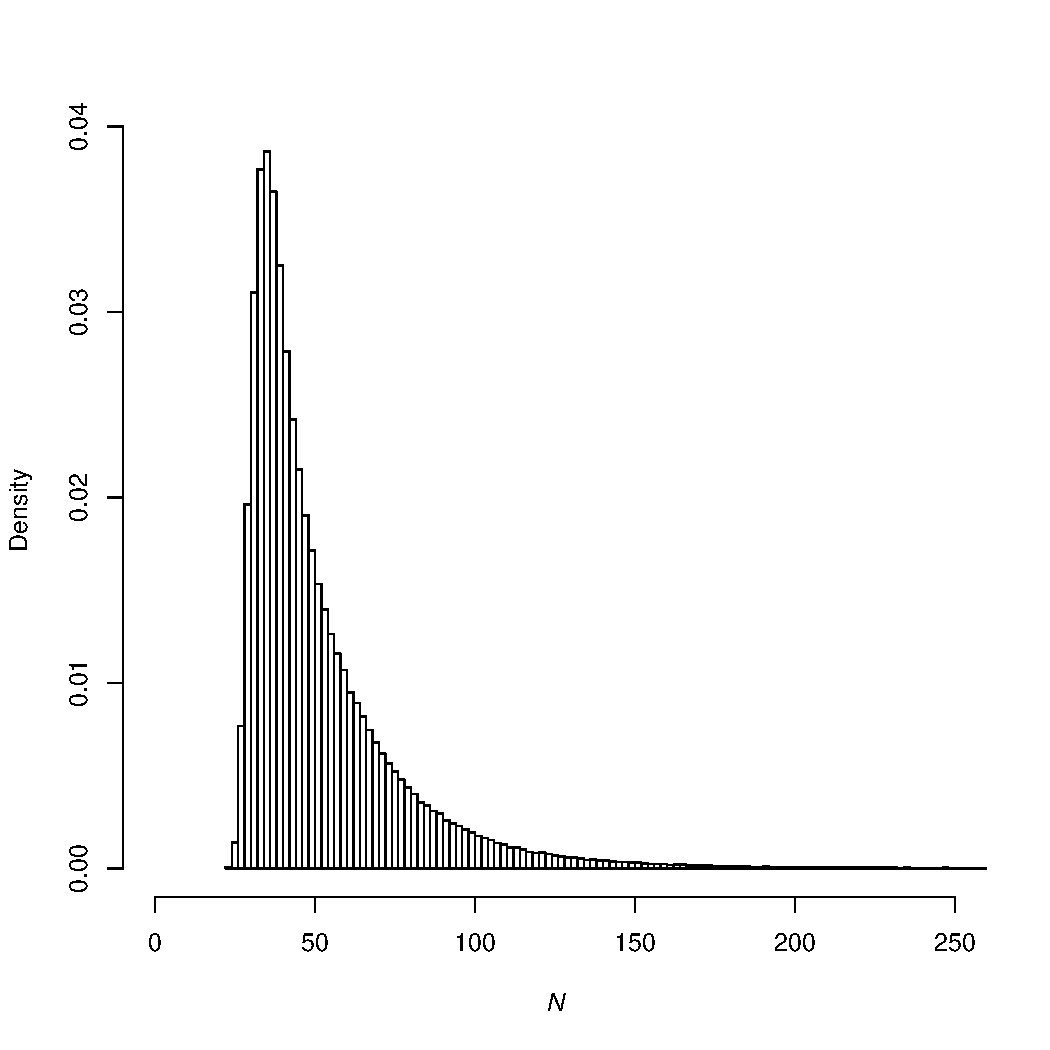
\includegraphics[width=6in,height=4in]{modaveN.pdf}
  \begin{doublespace}
    \caption{\label{fig:modaveN}Model-averaged posterior distribution of population abundance $(N)$ for the bobcat data.}
  \end{doublespace}
\end{figure}

\section{Discussion}
I have described some of the key features of \verb|multimark|, a new R package for the analysis of capture-recapture data with multiple non-invasive marks. The package adds to the growing toolbox of freely-available software for the analysis of non-spatial \citep[e.g.][]{WhiteBurnham1999,ChoquetEtAl2009,Laake2013,LaakeEtAl2013} and spatial \citep[e.g.][]{GopalaswamyEtAl2012,Efford2015} capture-recapture data, but it is the first to combine otherwise irreconcilable encounter histories arising from multiple mark types. Although initially developed for integrated analyses of left- and right-sided images for bilaterally asymmetrical species, the package can be used to jointly analyze data arising from any two types of marks. For example, \verb|multimark| could be used to integrate an analysis of encounter histories arising from genetic (e.g. hair or faecal) and visual (e.g. photo-ID) detections (sensu \citealt{MadonEtAl2011}; but see \citealt{Bonner2013}).

\verb|multimark| currently includes open population CJS and closed population models, with functions for derived parameters (e.g. $\phi$, $p$) and Bayesian multimodel inference. Relative to previous applications using multiple marks \citep{BonnerHolmberg2013,McClintockEtAl2013a}, the relatively fast computation times of the package are attributable to its use of ``semi-complete'' data likelihoods \citep{KingEtAl2015}, parallel processing, and MCMC algorithms written in C (instead of R). Because parallel processing relies on the \verb|parallel| package \citep{RTeam2013}, first-time Windows and OS X users can expect a firewall pop-up dialog box asking if an R process should accept incoming connections. Memory requirements are minimized by conditioning on the observed encounter histories when identifying the feasible set of latent encounter histories. To facilitate better mixing, \verb|multimark| extends the MCMC algorithms proposed by \cite{BonnerHolmberg2013} and \cite{McClintockEtAl2013a,McClintockEtAl2014} by avoiding latent encounter history proposals with negative frequencies in a manner that requires no proposal tuning (see Appendix S1 for details).

Many potentially desirable extensions to \verb|multimark| are possible. These include a broader suite of capture-recapture models, such as multi-state and robust design models \citep[e.g.][]{WilliamsEtAl2002}. In addition to individual-level heterogeneity, ``random effect'' distributions for temporal or user-specified covariates could also be incorporated \citep[e.g.][]{LaakeEtAl2013}. More general modelling formulae for ${\boldsymbol \delta}$ and $\alpha$ would allow additional hypotheses related to detection to be explored. The package could also be extended to accomodate >2 mark types and additional link functions. Although many individual covariates tend to be difficult (or impossible) to observe with non-invasive sampling, some (e.g. sex) may be easily discernable for each mark type. For these cases, it would be relatively straightforward to extend \verb|multimark| to accommodate individual covariates. Other extensions include spatially-explicit models \citep[e.g.][]{Royle2015} and allowing for partial overlap in the sampling periods for each mark type. Practitioners interested in such extensions are encouraged to contact the author.

\noindent \textbf{Acknowledgments} 

\noindent P. Boveng, P. Conn, and J. Laake for helpful comments on earlier drafts. D. Johnson for helpful discussions. The findings and conclusions in the manuscript are those of the author(s) and do not necessarily represent the views of the National Marine Fisheries Service, NOAA. Any use of trade, product, or firm names does not imply an endorsement by the US Government.

\bibliographystyle{mee}
\bibliography{master.bib}

\end{document}
